\documentclass{beamer}
%%%%%%%%%%%%%%%%%%%%%%%%%%%%%%%%%%%%%%%%%%%%%%%%%%%%%%%%%%%%%%%%%%%%%%%%%%%%
\usepackage{bm}
\usepackage{amsmath}
\usepackage{amssymb}
\usepackage{microtype}
\usepackage{booktabs} % \toprule, \midrule, \bottomrule
%%% INCLUDE FILE FOR DEFINITIONS
%%% These may require various packages.

% Shortcuts in regular text
\newcommand{\degs}{\ensuremath{^\circ}}
\newcommand{\EE}[1]{\ensuremath{\times 10^{#1}}}
\newcommand{\ttimes}{\ensuremath{{}\times{}}}
\newcommand{\cclicense}{%
  \smash{\raisebox{-0.45ex}{%
  \setlength{\unitlength}{1em}%
  \begin{picture}(1,1)%
    \put(0.5,0.5){\circle{1}}
    \put(0.5,0.5){\hbox to 0pt{\hss\raisebox{-.45ex}{\tiny\textsf{CC}}\hss}}
  \end{picture}%
  }}%
  \hskip -1em%
  \href{http://creativecommons.org/licenses/by-nc-sa/3.0/}%
  {\ \hskip 1em \textsf{BY-NC-SA}}%
}

%\newcommand{\horizsep}{{\par\noindent\centering\rule[.25ex]{.75\columnwidth}{2pt}\par}}
\newcommand{\horizsep}{\vspace{\baselineskip}\noindent\hspace{\stretch{1}}$
\ast\qquad \ast\qquad \ast\qquad
$ \hspace{\stretch{1}} \vspace{\baselineskip}}
\newcommand{\pytrt}{\textsf{PyTRT}}

% Research
\newcommand{\lop}[1]{\mathcal{L}\!\left[#1\right]}
\newcommand{\lopinv}[2]{\mathcal{I}_{#1}\!\left[#2\right]}
\newcommand{\Dtens}{\mat{D}}
\newcommand{\Etens}{\mat{E}}
\newcommand{\Identitytens}{\mat{I}}
\newcommand{\APone}{AP$_1$}
\newcommand{\Pone}{P$_1$}
\newcommand{\SN}{S$_N$}%{S$_\text{N}$}%{$S_N$}%
\newcommand{\PN}{P$_N$}%{P$_\text{N}$}%{$P_N$}%
\newcommand{\CN}{Crank--Nicolson} %Yes, it's Nic not Nich
\newcommand{\Eddington}{\mathcal{E}} %whatever symbol I decided for Eddington
\newcommand{\RadEn}{E} %whatever symbol I decide for radiation energy
\newcommand{\Sigmatr}{\Sigma_{\mathit{tr}}}

% Program names
\newcommand{\cpp}{\textsf{C\raisebox{0.2ex}{++}}}

% General math shortcuts
\newcommand{\ud}{\mathop{}\!\mathrm{d}}
\newcommand{\pder}[2]{\frac{\partial #1}{\partial #2}}
\newcommand{\oder}[2]{\frac{\mathrm{d} #1}{\mathrm{d} #2}}
\newcommand{\tpder}[2]{{\partial #1}/{\partial #2}} %inlined
\newcommand{\toder}[2]{{\mathrm{d} #1}/{\mathrm{d} #2}} %inlined
\newcommand{\lra}{ \quad \Longrightarrow \quad }
\newcommand{\eexp}{\mathop{}\!\mathrm{e}} % upright ``e'' for exponent
\newcommand{\expp}[1]{\exp\!\left( {#1} \right)} % exp with parentheses
\newcommand{\qeq}{\stackrel{\mathrm{?}}{=}}

% Probability
\newcommand{\expectation}[1]{\mathop{}\!\mathrm{E}\!\left[ #1 \right]}
\DeclareMathOperator{\Var}{Var} % variance

% Asymptotic analysis
\DeclareMathOperator{\Ei}{Ei} % Exponential function
\newcommand{\lapl}[1]{\mathcal{L}[{#1}]} %laplace

%change the Re and Im operators from fancy curly letters
\DeclareMathOperator{\MathOpRe}{Re}
\renewcommand{\Re}{\MathOpRe}
\DeclareMathOperator{\MathOpIm}{Im}
\renewcommand{\Im}{\MathOpIm}

%imaginary ``i'' , upright 'i' or \imath
\newcommand{\iimag}{\mathrm{i}}

% Finite differences
\newcommand{\hot}{\text{h.o.t.}}
\newcommand{\inv}{^{-1}}

% Numerical Linear Algebra
\newcommand{\conj}{^{\ast}} % complex conjugate (transpose)
\newcommand{\norm}[1]{\left\| #1 \right\|} % double pipe
\newcommand{\abs}[1]{\left| #1 \right|} % single pipe
\newcommand{\eps}{\varepsilon}
\DeclareMathOperator{\fl}{fl}

\DeclareMathOperator{\acosh}{arccosh} 

% Define a command to write a nice-looking element, e.g. 4,2 He
\newcommand{\elem}[3]{\ensuremath{{}^{{#1}}_{{#2}}\mathrm{{#3}}}}

% Vector definitions
\newcommand{\mat}[1]{\mathbf{#1}} %matrix is bold upright
\renewcommand{\vec}[1]{\bm{#1}} %vector is bold italic
\newcommand{\op}[1]{\mathsf{#1}} % ``operator'' is sans serif

\newcommand{\vd}{\bm{\cdot}} % slightly bold vector dot
\newcommand{\del}{\vec{\nabla}} % gradient (Del) is bold
\newcommand{\grad}{\vec{\nabla}} % gradient

%\newcommand{\abr}[1]{\langle {#1} \rangle}
\newcommand{\abr}[1]{\left\langle {#1} \right\rangle} % angle brackets for avg.

%% topbox is useful in extended definitions of math terms inside an align
\newcommand{\topbox}[2][0.6]{\parbox[t]{#1\columnwidth}{\raggedright{}#2}}

% commands to make text in math mode appear as zero-width (better-looking
% integrals/sums, e.g.)
% from mathmode.pdf page 74, or Alexander R. Perlis ``A complement to \smash,
% \llap, and \rlap''

\def\mathllap{\mathpalette\mathllapinternal}
	\def\mathllapinternal#1#2{%
	\llap{$\mathsurround=0pt#1{#2}$}%
}
\def\clap#1{\hbox to 0pt{\hss#1\hss}}%
\def\mathclap{\mathpalette\mathclapinternal}%
\def\mathclapinternal#1#2{%
	\clap{$\mathsurround=0pt#1{#2}$}%
}
\def\mathrlap{\mathpalette\mathrlapinternal}%
\def\mathrlapinternal#1#2{%
	\rlap{$\mathsurround=0pt#1{#2}$}%
}

\definecolor{lightgray}{gray}{0.85}
%%%%%%%%%%%%%%%%%%%%%%%%%%%%%%%%%%%%%%%%%%%%%%%%%%%%%%%%%%%%%%%%%%%%%%%%%%%%

%30 minute presentation
%15 minutes scheduled for questions
%1 hour allotted total

\usetheme{AnnArbor}
\usecolortheme{seahorse}
\usecolortheme{orchid}
\usefonttheme[onlymath]{serif}
\setbeamercolor*{frametitle}{use=structure,bg=structure.fg!20!white}
\setbeamercolor*{frametitle right}{use=structure,bg=structure.fg!20!white}
\setbeamertemplate{navigation symbols}{\insertframenavigationsymbol}
\setbeamertemplate{caption}[numbered]

\title[MC 2011]%
{An anisotropic diffusion approximation to nonlinear radiation transport}

\author[SRJ, EWL]{Seth~Johnson \and Ed~Larsen}

\institute[UMich]{
University of Michigan, Ann Arbor
}
\date[5/9/2011]{May 9, 2011}

\AtBeginSection[]
{
\begin{frame}
  \frametitle{Outline}
  \tableofcontents[currentsection]
\end{frame}
}

\hypersetup{colorlinks=true,linkcolor=black}

% only show section headings in table of contents
\setcounter{tocdepth}{1}

%use symbols for footnote
\renewcommand{\thefootnote}{\fnsymbol{footnote}}

\begin{document}
%%%%%%%%%%%%%%%%%%%%%%%%%%%%%%%%%%%%%%%%%%%%%%%%%%%%%%%%%%%%%%%%%%%%%%%%%%%%

\begin{frame}
\titlepage
\begin{center}
  
\includegraphics[width=0.2\textwidth]{../figures/umlogo}
\end{center}
\smash{
\includegraphics[width=0.2\textwidth]{../figures/neup-small}}
\end{frame}

%%%%%%%%%%%%%%%%%%%%%%%%%%%%%%%%%%%%%%%%%%%%%%%%%%%%%%%%%%%%%%%%%%%%%%%%%%%%
\section{Introduction}
%%%%%%%%%%%%%%%%%%%%%%%%%%%%%%%%%%%%%%%%
\begin{frame}
  \frametitle{Thermal radiative transfer}
  \begin{itemize}
    \item TRT is the dominant heat transfer process in very hot materials
    \item Photons born isotropically via black body emission
      ($q_\text{rad} \propto \sigma T^4$)
    \item Cold material heats up and becomes relatively transparent
      ($\sigma\propto T^{-3}$)
  \end{itemize}

  Difficulties in solving:
  \begin{itemize}
    \item High dimensionality of solution phase space $(\vec{x}, \vec{\Omega},
      h\nu, t)$
    \item Highly nonlinear coupled partial differential equations for radiation
      field $I(\vec{x}, \vec{\Omega}, h\nu, t)$ and material energy
  \end{itemize}

  Particular application of this work: CRASH project
  \begin{itemize}
    \item Center for RAdiative Shock Hydrodynamics program: ``Assessment
      of Predictive Capability''
    \item Simulate laser-driven shock in a xenon-filled tube
    \item Uncertainty quantification: hundreds of solution instances needed
  \end{itemize}
\end{frame}

%%%%%%%%%%%%%%%%%%%%%%%%%%%%%%%%%%%%%%%%
\begin{frame}
  \frametitle{Motivation}
\begin{center}
  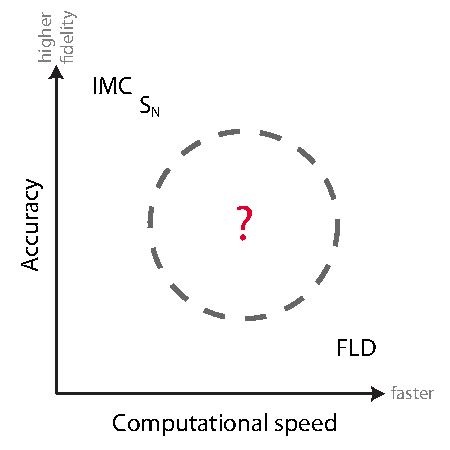
\includegraphics[width=3in]{../figures/fidelity}
\end{center}
% also, storage requirements
\end{frame}

%%%%%%%%%%%%%%%%%%%%%%%%%%%%%%%%%%%%%%%%
\begin{frame}
  \frametitle{Gray TRT equations}
  Common approximations for radiation transport methods development:
  \begin{itemize}
    \item work in a fixed medium, disregarding material advection;
    \item assume local thermodynamic equilibrium (LTE), which uses a single
      material temperature;
    \item neglect thermal conduction in material;
    \item average over all photon energies $h\nu$ (gray).
  \end{itemize}
\begin{subequations} \label{eqs:fullGrayTRT}
  Radiation transfer equation, intensity $I(\vec{x}, \vec{\Omega}, t)$:
\begin{equation} \label{eq:fullGrayTransport}
  \frac{1}{c} \pder{I}{t}
  + \vec{\Omega} \vd \del I +
 \sigma I
  = \frac{\sigma c aT^4}{4\pi} 
  + \frac{c Q}{4\pi}
\end{equation}
  Material energy balance equation:
\begin{equation} \label{eq:fullGrayMaterial}
  \frac{1}{c_v}\pder{T}{t} = \sigma \int_{4\pi}  I \ud\Omega - \sigma c aT^4
\end{equation}
\end{subequations}
\end{frame}

%%%%%%%%%%%%%%%%%%%%%%%%%%%%%%%%%%%%%%%%
\begin{frame}
  \frametitle{Anisotropic diffusion}
  Previous work:
  \begin{itemize}
    \item Steady-state infinite medium VHTR-like problem with analytically
      calculated coefficients \cite{Lar2009c}
    \item Non-local tensor diffusion \cite{Mor2007} for steady-state
      radiative transfer, no further development or analysis in literature
  \end{itemize}
  Current work:
  \begin{itemize}
    \item Uses transport-calculated anisotropic diffusion tensors
    \item Applies to nonlinear, time-dependent problems with isotropic sources
  \end{itemize}
  Potential applications:
  \begin{itemize}
    \item Extends diffusion theory to new regimes of applicability
    \item Variance reduction with shielding problems that have voids
  \end{itemize}
\end{frame}

%%%%%%%%%%%%%%%%%%%%%%%%%%%%%%%%%%%%%%%%%%%%%%%%%%%%%%%%%%%%%%%%%%%%%%%%%%%%
\section{Theory}
%%%%%%%%%%%%%%%%%%%%%%%%%%%%%%%%%%%%%%%%
\begin{frame}{Summary in advance (infinite medium)}
\begin{enumerate}
  \item Define the anisotropic intensity as $\Psi = I - \frac{1}{4\pi}\phi$.
    We will approximate $\Psi$ rather than $I$.
  \item From the radiation transport equation and conservation equation, we get
    a differential transport equation for $\Psi$. Transform this to an integral
    transport equation for $\Psi$.
  \item Assume $I=O(1)$, $\frac1c\pder{}{t}=O(\epsilon^2)$, $\grad =
    O(\epsilon)$, $\int_{4\pi} \vec{\Omega} (\cdot) \ud\Omega = O(\epsilon)$.
  \item Use Taylor series to approximate nonlocal unknowns with local
    unknowns, discarding small terms. This yields
    \begin{equation*}
      \Psi(\vec{x}, \vec{\Omega})
      \approx - f(\vec{x}, \vec{\Omega})  \vec{\Omega} \vd \grad \phi\,.
    \end{equation*}
  \item Take the first angular moment of $\Psi$ to get $\vec{F}=-\Dtens \vd
    \grad \phi$
  \item Substitute $\vec{F}$ into the time-dependent particle
    conservation equation to get time-dependent anisotropic diffusion.
\end{enumerate}
\end{frame}

\subsection{Anisotropic diffusion derivation}
%%%%%%%%%%%%%%%%%%%%%%%%%%%%%%%%%%%%%%%%
\begin{frame}{Transport equation}
  Inside a time step, with ``frozen'' opacities:
\begin{subequations} \label{eqs:fullTransport}
\begin{multline} \label{eq:fullTransportVol}
  \frac{1}{c} \pder{I}{t}(\vec{x}, \vec{\Omega}, t)
    + \vec{\Omega}\vd \grad I(\vec{x}, \vec{\Omega}, t)
    + \sigma^\ast(\vec{x}) I (\vec{x}, \vec{\Omega}, t)
    \\
    = \frac{1}{4\pi} \sigma^\ast(\vec{x}) ac [T(\vec{x}, t)]^4
    + \frac{1}{4\pi} q_{r}(\vec{x}, t)
    \equiv \frac{1}{4\pi} Q(\vec{x}, t) \,,
\\
x \in V,\  0 \le t < \Delta_t, \ \vec{\Omega} \in 4\pi,
\end{multline}
and the initial condition
\begin{equation} \label{eq:fullTransportInit}
 I(\vec{x}, \vec{\Omega}, 0) = I^i(\vec{x}, \vec{\Omega}, t) \,,
 \quad \vec{x} \in V, \ \vec{\Omega} \in 4\pi\,.
\end{equation}
\end{subequations}
For this presentation, only consider an infinite (non-homogeneous) medium.
\end{frame}

%%%%%%%%%%%%%%%%%%%%%%%%%%%%%%%%%%%%%%%%
\begin{frame}{Conservation equations}
Operating on Eq.~\eqref{eq:fullTransportVol} by $\int_{4\pi} (\cdot) \ud\Omega$
gives
\begin{subequations} \label{eqs:loEquations}
\begin{equation} \label{eq:loVol}
\frac{1}{c} \pder{\phi}{t} (\vec{x}, t)
  + \grad \vd\vec{F}(\vec{x}, t)
  + \sigma^\ast \phi(\vec{x}, t)
  =  Q(\vec{x}, t)\,.
\end{equation}
and on the initial condition, Eq.~\eqref{eq:fullTransportInit},
\begin{equation} \label{eq:loInit}
\phi(\vec{x}, 0) = \int_{4\pi}  I^i(\vec{x},
\vec{\Omega}) \ud\Omega = \phi^i(\vec{x}) \,.
\end{equation}
\end{subequations}

Add $\vec{\Omega}\vd\grad \phi$ to both sides of Eq.~\eqref{eq:loVol} and
multiply by $\frac{1}{4\pi}$:
\begin{equation} \label{eq:modifiedConservation}
  \frac{1}{4\pi} \frac{1}{c} \pder{\phi}{t}
  + \frac{1}{4\pi} \vec{\Omega}\vd\grad \phi
  + \frac{1}{4\pi} \sigma^\ast \phi
  = \frac{1}{4\pi}  Q(\vec{x}, t) + \frac{1}{4\pi} \vec{\Omega}\vd\grad \phi
  - \frac{1}{4\pi} \grad \vd\vec{F}
\end{equation}
\end{frame}

%%%%%%%%%%%%%%%%%%%%%%%%%%%%%%%%%%%%%%%%
\begin{frame}{Anisotropic intensity equations}
  Define ``anisotropic intensity'':
  \begin{equation} \label{eq:capPsi}
    \Psi(\vec{x}, \vec{\Omega}) \equiv I(\vec{x}, \vec{\Omega})
    - \frac{1}{4\pi} \phi(\vec{x})\,.
  \end{equation}
  (This satisfies $\int_{4\pi} \Psi=0$ and $\int_{4\pi} \vec{\Omega} \Psi =
  \vec{F}$.)

  Subtract Eq.~\eqref{eq:modifiedConservation} from
  Eq.~\eqref{eq:fullTransportVol}; the isotropic source cancels:
\begin{multline*}
  \frac{1}{c} \pder{}{t} \left[ I - \frac{\phi}{4\pi} \right]
    + \vec{\Omega}\vd \grad \left[ I - \frac{\phi}{4\pi} \right]
    + \sigma^\ast(\vec{x})\left[ I - \frac{\phi}{4\pi} \right]
  = \frac{1}{4\pi} \grad \vd\vec{F} -
  \frac{1}{4\pi} \vec{\Omega}\vd \grad \phi
\end{multline*}
\begin{equation*}
  \frac{1}{c} \pder{}{t} \Psi
   + \vec{\Omega}\vd \grad \Psi
   + \sigma^\ast(\vec{x}) \Psi
  = \frac{1}{4\pi} \grad \vd\vec{F} -
  \frac{1}{4\pi} \vec{\Omega}\vd \grad \phi
  \equiv \hat Q(\vec{x}, \vec{\Omega}, t)
\end{equation*}

  Subtract Eq.~\eqref{eq:loInit} from Eq.~\eqref{eq:fullTransportInit}:
  \begin{equation*}
    \Psi(\vec{x}, \vec{\Omega}, 0) =
    I(\vec{x}, \vec{\Omega}, 0) - \frac{1}{4\pi}\phi(\vec{x}, 0)
    = I^i - \frac{\phi^i}{4\pi}
  \end{equation*}
  The exact solutions for $I$, $\phi$, $\vec{F}$ satisfy these equations: still
  no approximations.
\end{frame}

%%%%%%%%%%%%%%%%%%%%%%%%%%%%%%%%%%%%%%%%
\begin{frame}{Integral transport equation}
  Streaming path from $(\vec{x}, t)$ backward along $-\vec{\Omega}$, accumulate
  sources and attenuate:
\begin{subequations} \label{eqs:inverseTransport}
  \begin{align} \label{eq:inverseTransportFull}
  \begin{split}
    \Psi(\vec{x}, \vec{\Omega}, t)
    &=
    \Psi^i( \vec{x} - ct \vec{\Omega}, \vec{\Omega})
    \eexp^{ -\tau(\vec{x}, \vec{x} - ct \vec{\Omega})}
    \\
    &\qquad + \int_{0}^{\infty}
    \left[ \hat Q(\vec{x} - s \vec{\Omega}, \vec{\Omega}, t-s/c)
    \right]
    \eexp^{ -\tau(\vec{x}, \vec{x} - s \vec{\Omega})}
    \ud s\,.
  \end{split}
    \\ 
    &\equiv  \lopinv{i}{\Psi^i}
    + \lopinv{v}{\hat Q}
    \\ \nonumber
    &= \lopinv{i}{\Psi^i}
  + \lopinv{v}{\frac{1}{4\pi} \grad \vd\vec{F}} -
  \lopinv{v}{\frac{1}{4\pi} \vec{\Omega}\vd \grad \phi} \,.
  \end{align}
  Here, the optical thickness is 
  \begin{equation} \label{eq:fullTauDefinition}
    \tau(\vec{x}, \vec{x}') = \int_{0}^{\abs{\vec{x} -
    \vec{x}'}} \sigma^\ast(\vec{x}-s\vec{\Omega}) \ud s \,.
  \end{equation}
\end{subequations}
These are nonlocal unknowns; we will approximate them with local unknowns.
\end{frame}

%%%%%%%%%%%%%%%%%%%%%%%%%%%%%%%%%%%%%%%%
\begin{frame}{Time for some approximations}
  Asymptotic ansatz: assume weak spatial gradients, mildly anisotropic intensity, very small time
  derivative:
\begin{align*}
  I &= O(1), &
  \del I &= O(\epsilon)&
  \int_{4\pi} \vec{\Omega} I\ud\Omega &= O(\epsilon)&
  \frac{1}{c} \pder{}{t} &= O(\epsilon^2)
\end{align*}

Our first approximation: $\lopinv{i}{\cdot} = O(\epsilon^2)$ and $\grad \vd \vec{F} =
O(\epsilon^2)$:
\begin{align*}
  \Psi &= \lopinv{i}{\Psi^i}
  + \lopinv{v}{\frac{1}{4\pi} \grad \vd\vec{F}} -
  \lopinv{v}{\frac{1}{4\pi} \vec{\Omega}\vd \grad \phi}
    \\ 
  \Psi 
  &\approx - \lopinv{v}{\frac{1}{4\pi} \vec{\Omega}\vd \grad \phi}
  + O(\epsilon^2)
\end{align*}

Taylor series expansion:
\begin{align} \nonumber
  \phi(\vec{x} - s\vec{\Omega}, t - s/c)
  &\sim \phi(\vec{x}, t)
  - s \bigg( \frac{1}{c} \pder{}{t} + \vec{\Omega} \vd \grad \bigg)
  \phi(\vec{x}, t) + O(\epsilon^2)
\\ \label{eq:taylorPhi}
\phi(\vec{x} - s\vec{\Omega}, t - s/c)
&= \phi(\vec{x}, t) + O(\epsilon)
\end{align}
\end{frame}

%%%%%%%%%%%%%%%%%%%%%%%%%%%%%%%%%%%%%%%%
\begin{frame}{Internal approximation to $\Psi$}
  Applying the Taylor series expansion under the assumption of a smooth $\phi$,
  \begin{align*}
  -\lopinv{v}{ \frac{1}{4\pi} \vec{\Omega}\vd \grad \phi }
  &= -\int_{0}^{\infty}
    \left[ \frac{1}{4\pi} \vec{\Omega}\vd \grad \phi \right]_{(\vec{x} - s
    \vec{\Omega}, t-s/c)}
    \eexp^{ -\tau(\vec{x}, \vec{x} - s \vec{\Omega})}
    \ud s
  \\\nonumber
  &\sim - \int_{0}^{\infty}
    \left[ \frac1{4\pi}\right]
    \eexp^{ -\tau(\vec{x}, \vec{x} - s \vec{\Omega})} \ud s
    \vec{\Omega}\vd \grad \phi(\vec{x},t) + O(\epsilon^2)
  \\\label{eq:tildeS}
  &= - \lopinv{v}{ \frac1{4\pi} } \vec{\Omega}\vd \grad \phi(\vec{x},t)
  %&\equiv -f(\vec{x}, \vec{\Omega}) \vec{\Omega}\vd \grad \tilde
  %\phi(\vec{x},t)
  \end{align*}
  where $ \lopinv{v}{ \frac1{4\pi} } \equiv f$ is the solution to a purely
  absorbing transport equation:
\begin{subequations} \label{eqs:fFull}
  \begin{equation} \label{eq:fFullVol}
    \vec{\Omega}\vd \grad f(\vec{x}, \vec{\Omega})
    + \sigma^\ast f (\vec{x}, \vec{\Omega})
  =  \frac{1}{4\pi} \,, \quad x \in V,\ \vec{\Omega} \in 4\pi\,,
  \end{equation}
\begin{equation} \label{eq:fFullBndy}
  f(\vec{x}, \vec{\Omega}) = 0 \,,
 \quad \vec{x} \in \partial V, \ \vec{\Omega} \vd \vec{n} < 0 \,.
\end{equation}
\end{subequations}
\end{frame}

%%%%%%%%%%%%%%%%%%%%%%%%%%%%%%%%%%%%%%%%
\begin{frame}{An analogy to Fick's Law}
  To get an expression for the radiation flux (a.k.a.~``current''), use the identity
  $\vec{F} = \int_{4\pi}\vec{\Omega} \Psi \ud\Omega$,
  \begin{align*}
    \vec{F}(\vec{x}, t)
    &= \int_{4\pi}\vec{\Omega} \left( - \lopinv{v}{
    \frac1{4\pi} } \vec{\Omega}\vd \grad \phi(\vec{x},t) \right)
    \ud\Omega
    \\
      &= - \left[ \int_{4\pi}\vec{\Omega}\vec{\Omega} f \ud\Omega\right] \vd \grad \phi
    \\
      &\equiv -\Dtens \vd \grad \phi \,.
  \end{align*}

  Substitute into radiation energy conservation equation:
\begin{equation*}
  \frac{1}{c} \pder{\phi}{t}
  + \del \vd \vec{F} + \textcolor{red}{\sigma^*} \phi
  = \textcolor{red}{\sigma} ac\textcolor{red}{T^4}
  + c Q
\end{equation*}
Couple with the material energy balance equation:
\begin{equation*}
  \frac{1}{\textcolor{red}{c_v}}\pder{T}{t} = \textcolor{red}{\sigma^*} \phi -
  \textcolor{red}{\sigma^*} ac\textcolor{red}{T^4}
\end{equation*}
Approximate the red terms semi-implicitly.

\end{frame}

\subsection{Anisotropic diffusion discussion}
%%%%%%%%%%%%%%%%%%%%%%%%%%%%%%%%%%%%%%%%
\begin{frame}
  The transport problem used to calculate $\Dtens$,
  \begin{equation*}
    \vec{\Omega}\vd \del f + \sigma^* f = \frac{1}{4\pi} \,,
  \end{equation*}
  \vspace{-\baselineskip}
  \begin{itemize}
    \item Takes only one transport sweep to solve, since it is the description
      of a purely absorbing medium
    \item Only needs to be calculated once per time step (because of changing
      $\sigma^*$) in a nonlinear problem \item Requires no storage of the
      angular intensity, just accumulation of second moment, $D_{ij} =
      \int_{4\pi} \Omega_i \Omega_j f \ud\Omega$
    \item Has the solution $f=1/4\pi\sigma$ if $\sigma$ is a constant.
      Then, $\int_{4\pi} \vec{\Omega} f \vec{\Omega} \ud\Omega =
      \mat{I}/3\sigma$.
    \item For a finite medium, we must derive boundary conditions.
  \end{itemize}
\end{frame}

%%%%%%%%%%%%%%%%%%%%%%%%%%%%%%%%%%%%%%%%
\begin{frame}
  \frametitle{Properties of anisotropic diffusion}

  The anisotropic diffusion tensor $\Dtens(\vec{x},t)$: 
  \begin{itemize}
    \item Results from consistent approximations to the transport equation
      using physical coefficients
    \item Reduces to $\mat{I}/3\sigma$ for infinite homogeneous
      medium, which gives standard diffusion solution
    \item Has a greater ``action'' along the direction of a voided channel than
      across it (see later visualization)
    \item Does not ``blow up'' in void regions
    \item Is continuous in $\vec{x}$, so the approximate AD-calculated $\phi$
      has continuous first derivatives (i.e., $\phi$ is smooth like our ansatz
      requires)
  \end{itemize}
\end{frame}

%%%%%%%%%%%%%%%%%%%%%%%%%%%%%%%%%%%%%%%%%%%%%%%%%%%%%%%%%%%%%%%%%%%%%%%%%%%%
\section{Results}
%%%%%%%%%%%%%%%%%%%%%%%%%%%%%%%%%%%%%%%%
\begin{frame}{Compared methods}
\begin{itemize}
  \item Implicit Monte Carlo \cite{Fle1971} (implemented with variance
    reduction methods), $10^7$ particles per time step
  \item Flux-limited diffusion with Larsen limiter \cite{Ols2000}, with
    semi-implicit treatment of diffusion coefficient and radiation:
    \begin{equation*}
      \vec{F}^{n+1} = - D^{n} \del \phi^{n+1}  = -\left[ (3\sigma^{n})^2
      + \left( \frac{\abs{\del \phi^{n}}}{\phi^{n}}  \right)^2 \right]^{-1/2}
      \del \phi^{n+1}
    \end{equation*}
  \item Standard diffusion, with semi-implicit treatment of nonlinearities:
    \begin{equation*}
      \vec{F}^{n+1} = - D^{n} \del \phi^{n+1} 
      = -\frac{1}{3\sigma^{n}} \del \phi^{n+1}
    \end{equation*}
  \item Anisotropic diffusion, with semi-implicit treatment of nonlinearities:
    \begin{equation*}
      \vec{F}^{n+1} = -\Dtens^{n}\vd \del \phi^{n+1} 
    \end{equation*}
\end{itemize}
\end{frame}

%%%%%%%%%%%%%%%%%%%%%%%%%%%%%%%%%%%%%%%%
\begin{frame}
  \frametitle{AD implementation}
  \begin{block}{Approximations in the theory}
    \begin{itemize}
      \item Assume weak gradients and angular moments for $I$ (\emph{don't}
        assume that $I$ is a linear function of $\vec{\Omega}$!)
      \item Apply semi-implicit approximation for nonlinear material coupling
        and radiation
    \end{itemize}
  \end{block}
  \vspace{-\baselineskip}
  \begin{columns}[t]
    \begin{column}{.48\textwidth}
\begin{block}{$\Dtens$ transport equation}
  \begin{itemize}
    \item \SN\ angular approximation
    \item DD spatial approximation
  \end{itemize}
\end{block}
    \end{column}
    \begin{column}{.48\textwidth}
\begin{block}{AD equation}
  \begin{itemize}
    \item 9-point cell-centered finite difference spatial approximation
  \end{itemize}
\end{block}
    \end{column}
  \end{columns}
\end{frame}

%%%%%%%%%%%%%%%%%%%%%%%%%%%%%%%%%%%%%%%%%%%%%%%%%%%%%%%%%%%%%%%%%%%%%%%%%%%%
\subsection{Test problem}
%%%%%%%%%%%%%%%%%%%%%%%%%%%%%%%%%%%%%%%%
\begin{frame}{Problem description}
  \begin{columns}[t]
    \begin{column}{.48\textwidth}
      Flatland geometry!
      \\Uniform spatial grid: $\Delta_x=0.1$
      \\Piecewise linear time grid: $\Delta_t=0.1$ for $t \ge 1$
      \\Reflecting bndy on left, others vacuum
    \end{column}
    \begin{column}{.48\textwidth}
      \textcolor[rgb]{0,0,1}{\textbf{Source}}: $c_v=0.5$, $\sigma=0.5$;
      $Q=1$ for $0 \le t \le 1$, $Q=0$ for $t > 1$.

      \textcolor[rgb]{1,0,0}{\textbf{Diffusive}}: $c_v=0.1$,
      $\sigma=T^{-3}$

      \textcolor[rgb]{0.1,0.9,0.1}{\textbf{Channel}}: $c_v=0.1$,
      $\sigma=0.01 T^{-3}$

      Initial condition: $T=T_\text{rad}=0.1$
    \end{column}
  \end{columns}
\begin{center}
  \includegraphics[width=.99\textwidth]{../figures/crashpipe2/materials}
\end{center}
\end{frame}

%%%%%%%%%%%%%%%%%%%%%%%%%%%%%%%%%%%%%%%%
\begin{frame}{Time evolution of material temperature}
\only<1>{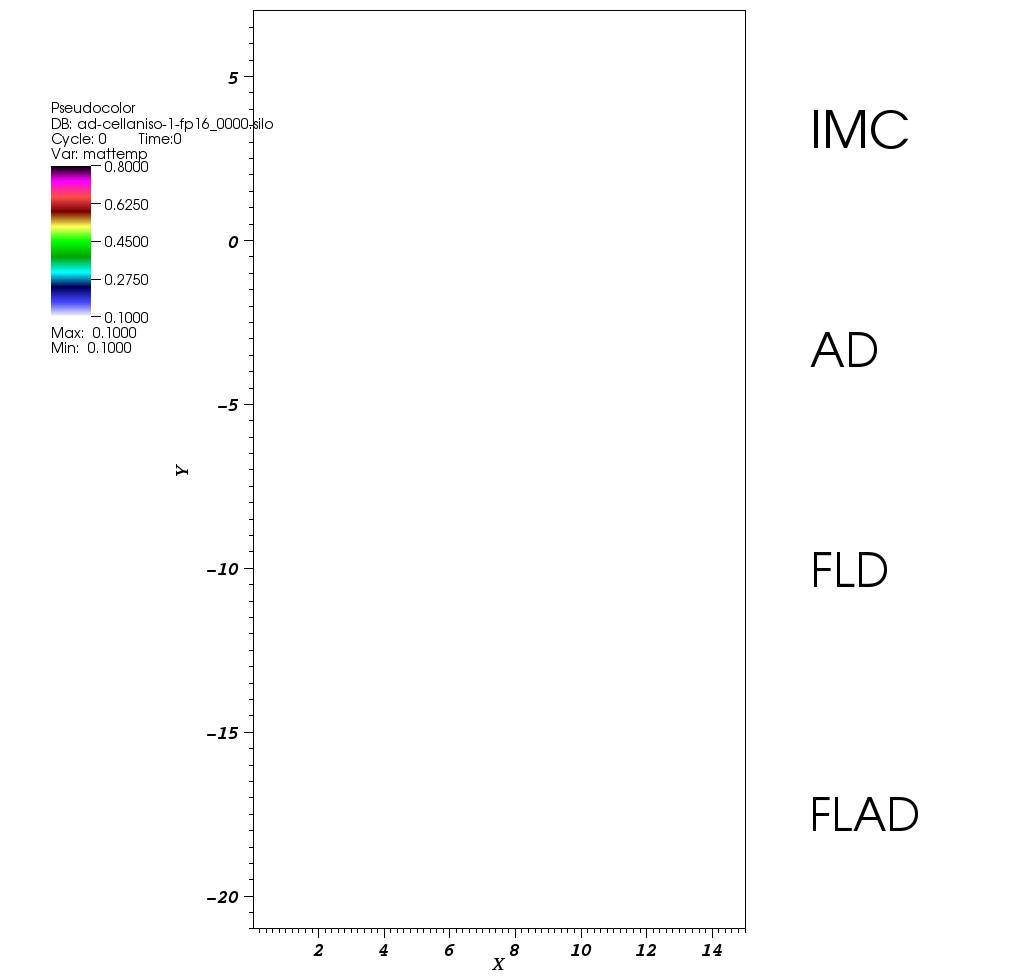
\includegraphics[height=3in]{../figures/crashpipe2b/mattemp/0000}$t=0$}%
\only<2>{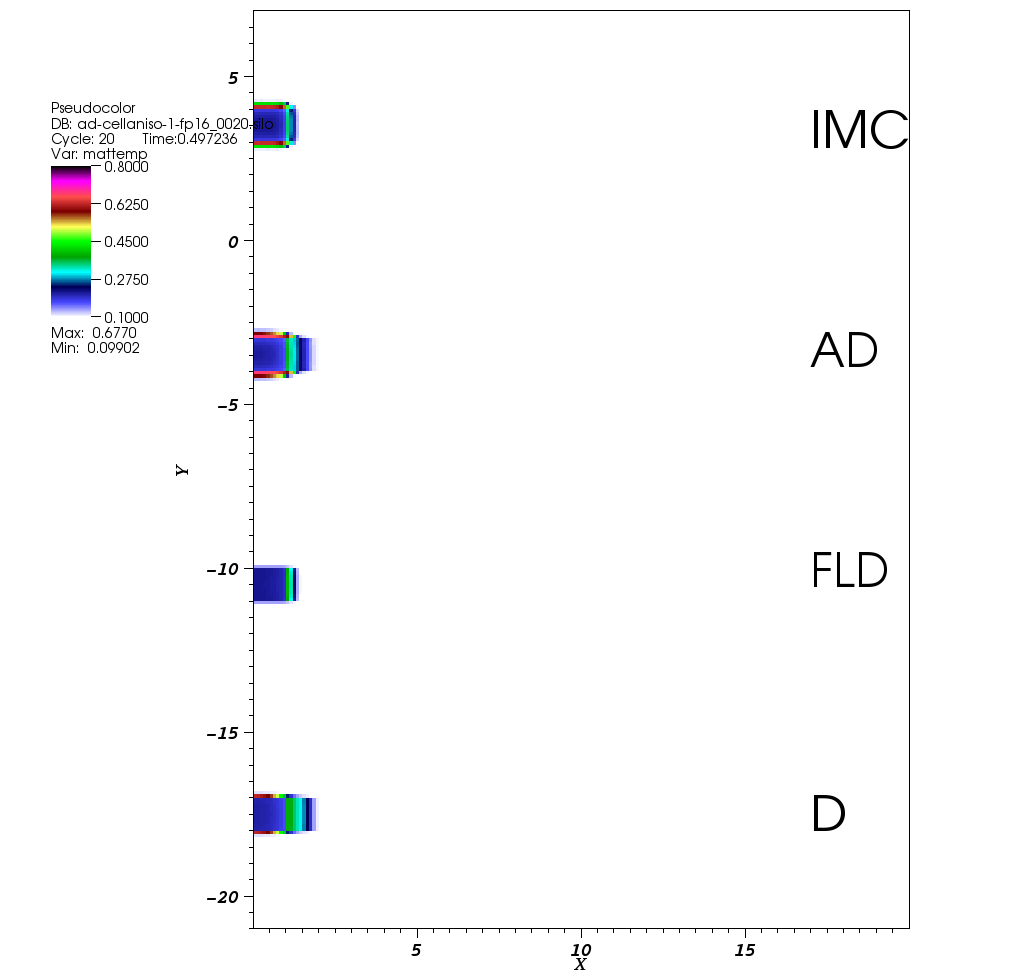
\includegraphics[height=3in]{../figures/crashpipe2b/mattemp/0020}$t=0.5$}%
\only<3>{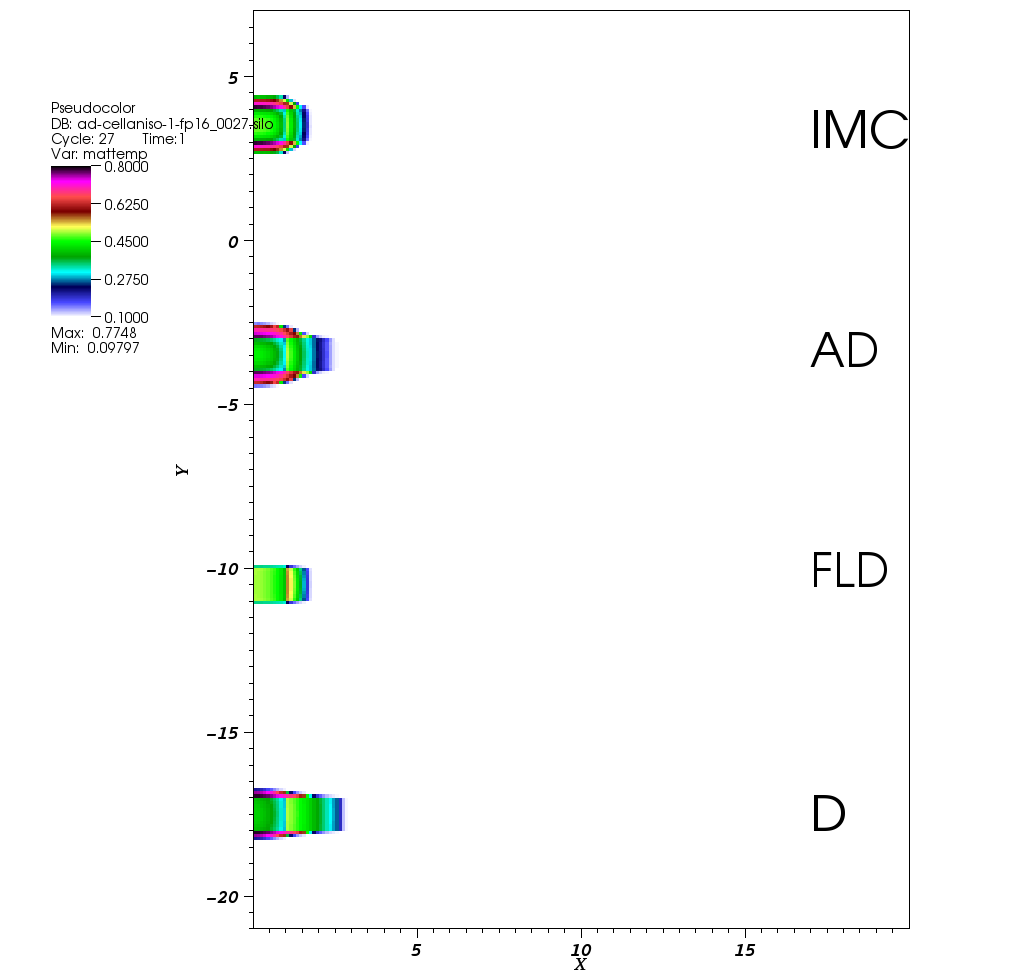
\includegraphics[height=3in]{../figures/crashpipe2b/mattemp/0027}$t=1.0$}%
\only<4>{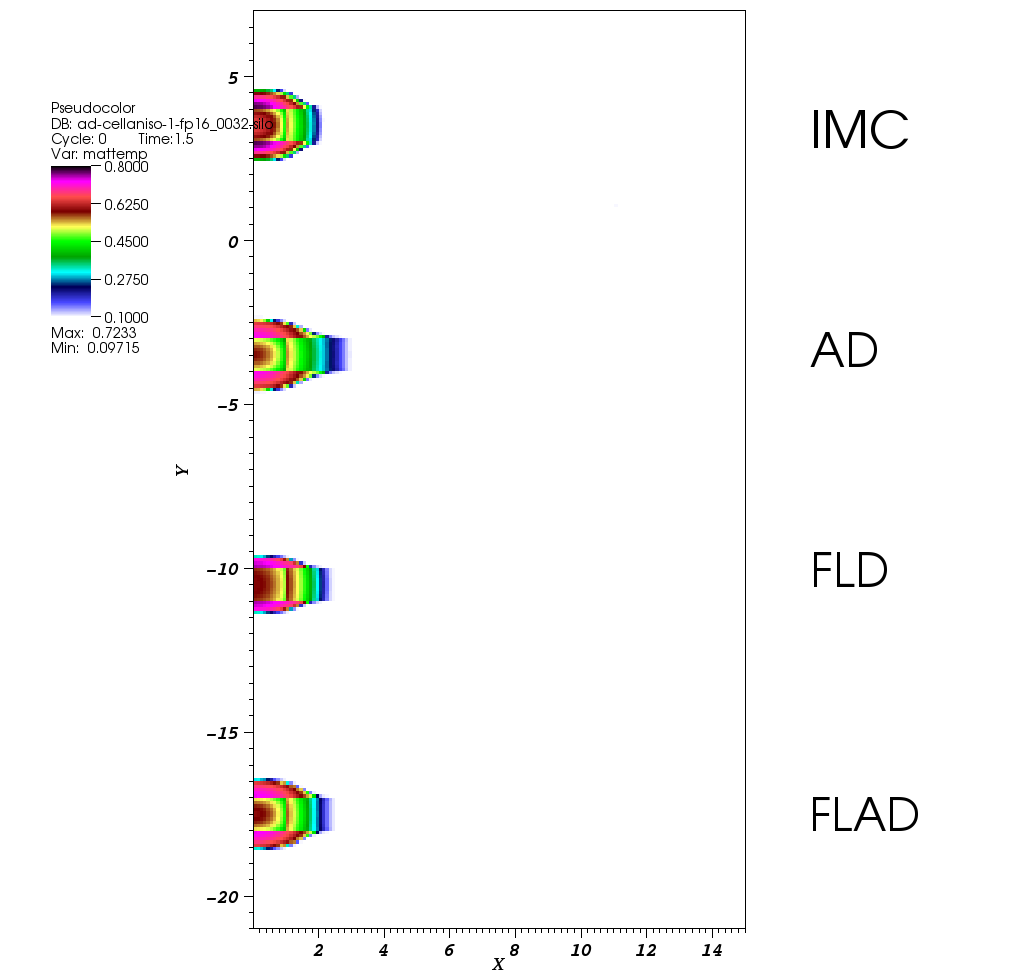
\includegraphics[height=3in]{../figures/crashpipe2b/mattemp/0032}$t=1.5$}%
\only<5>{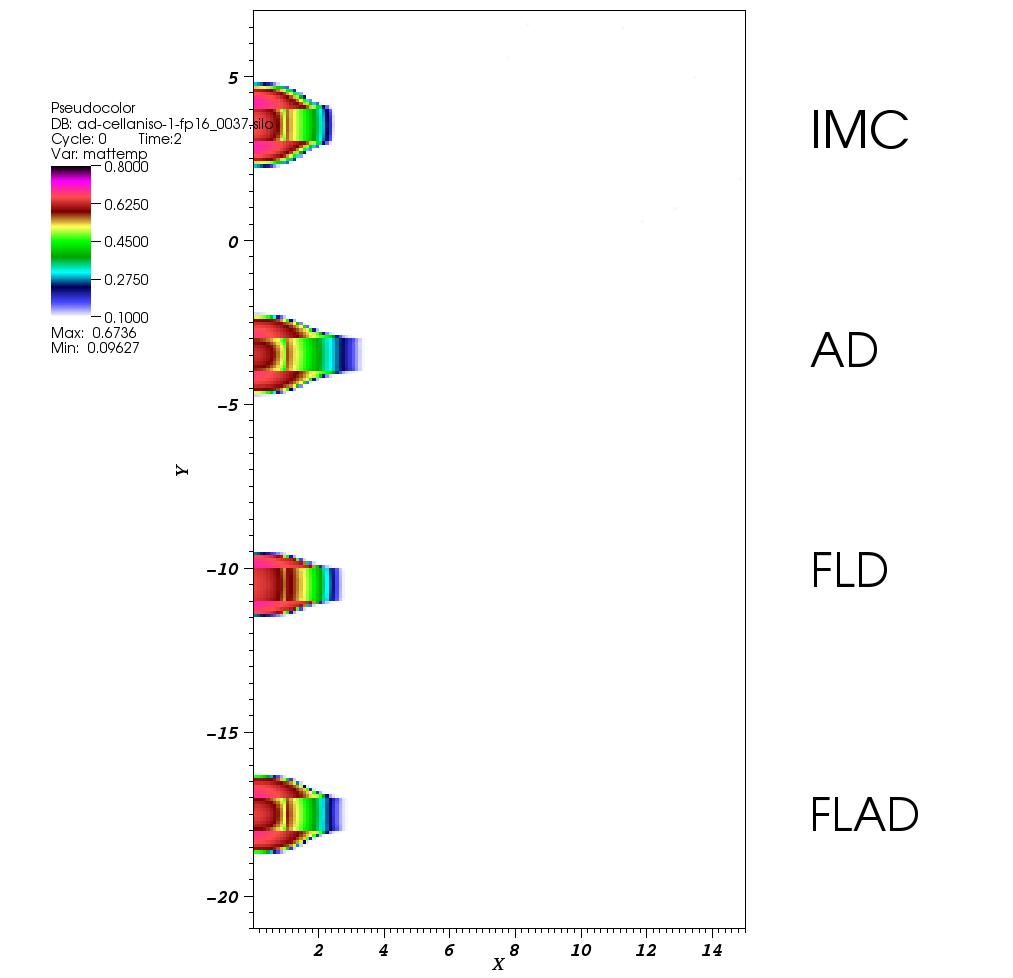
\includegraphics[height=3in]{../figures/crashpipe2b/mattemp/0037}$t=2$}%
\only<6>{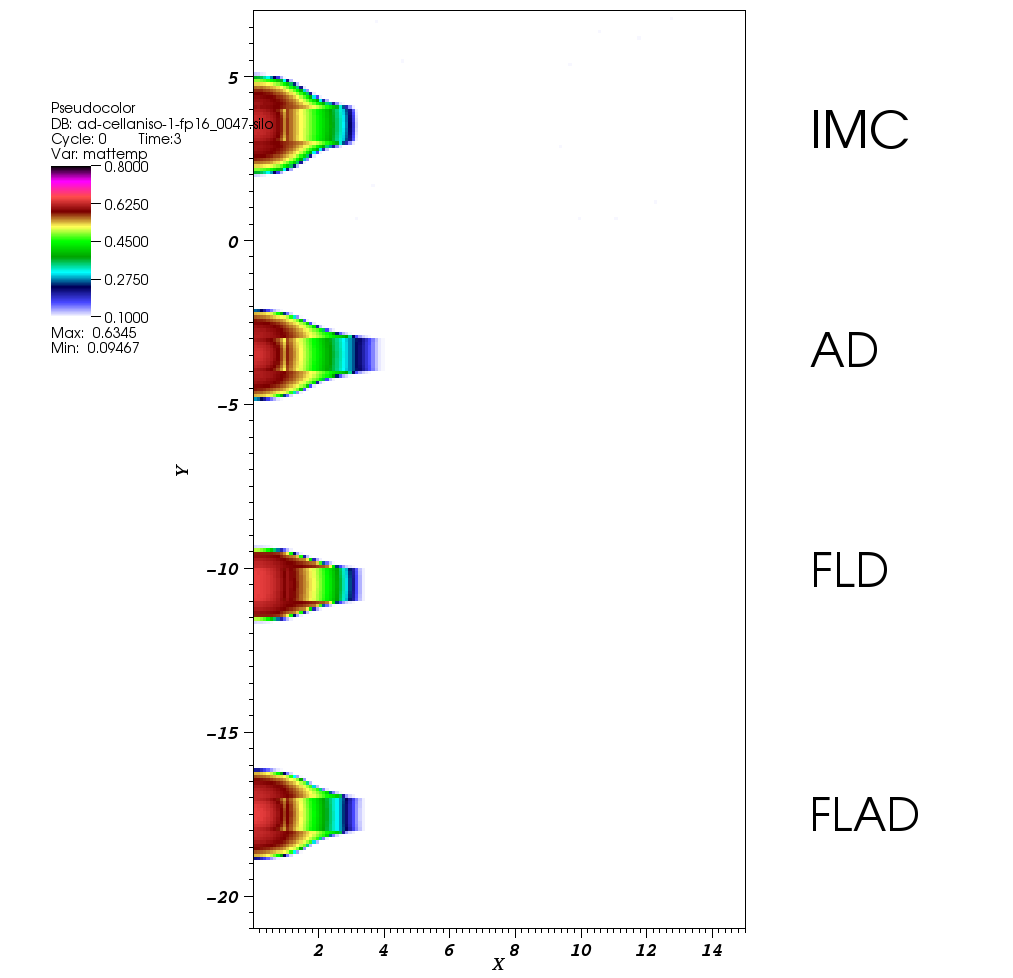
\includegraphics[height=3in]{../figures/crashpipe2b/mattemp/0047}$t=3$}%
\only<7>{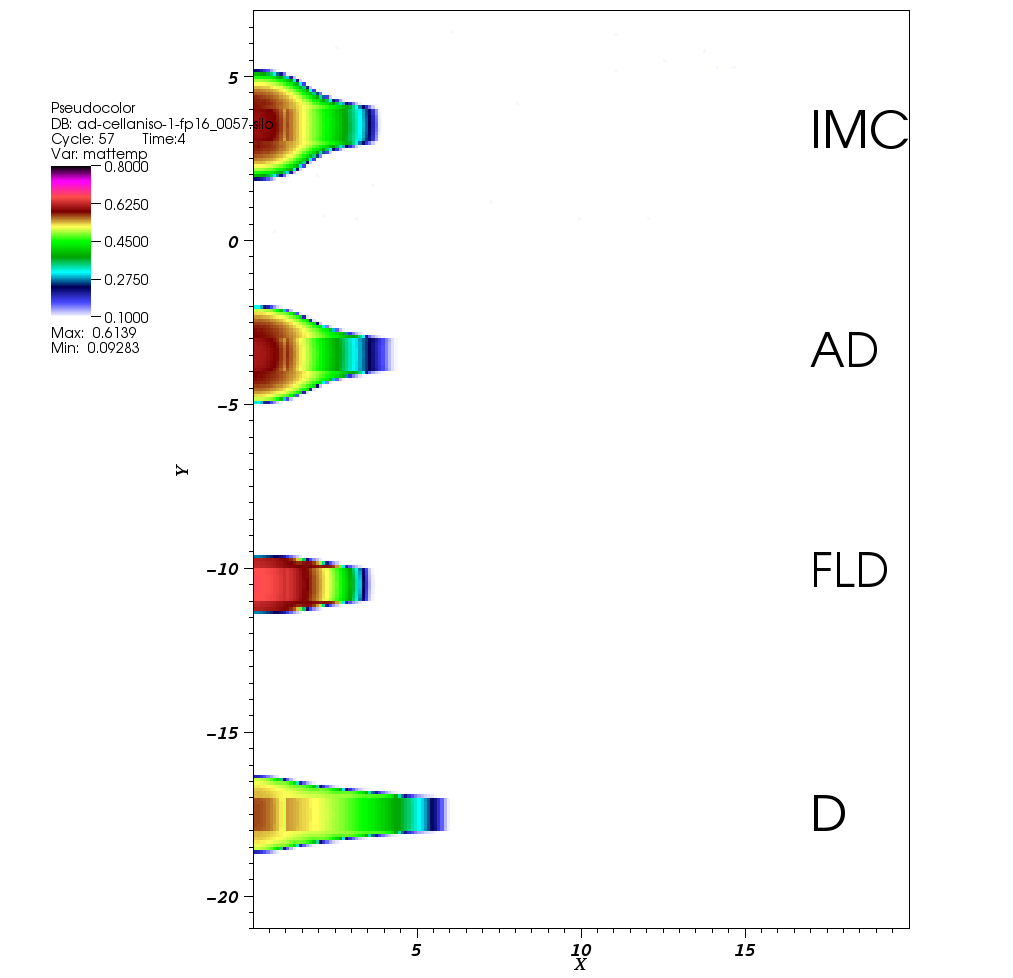
\includegraphics[height=3in]{../figures/crashpipe2b/mattemp/0057}$t=4$}%
\only<8>{\includegraphics[height=3in]{../figures/crashpipe2b/mattemp/0067}$t=5$}%
\only<9>{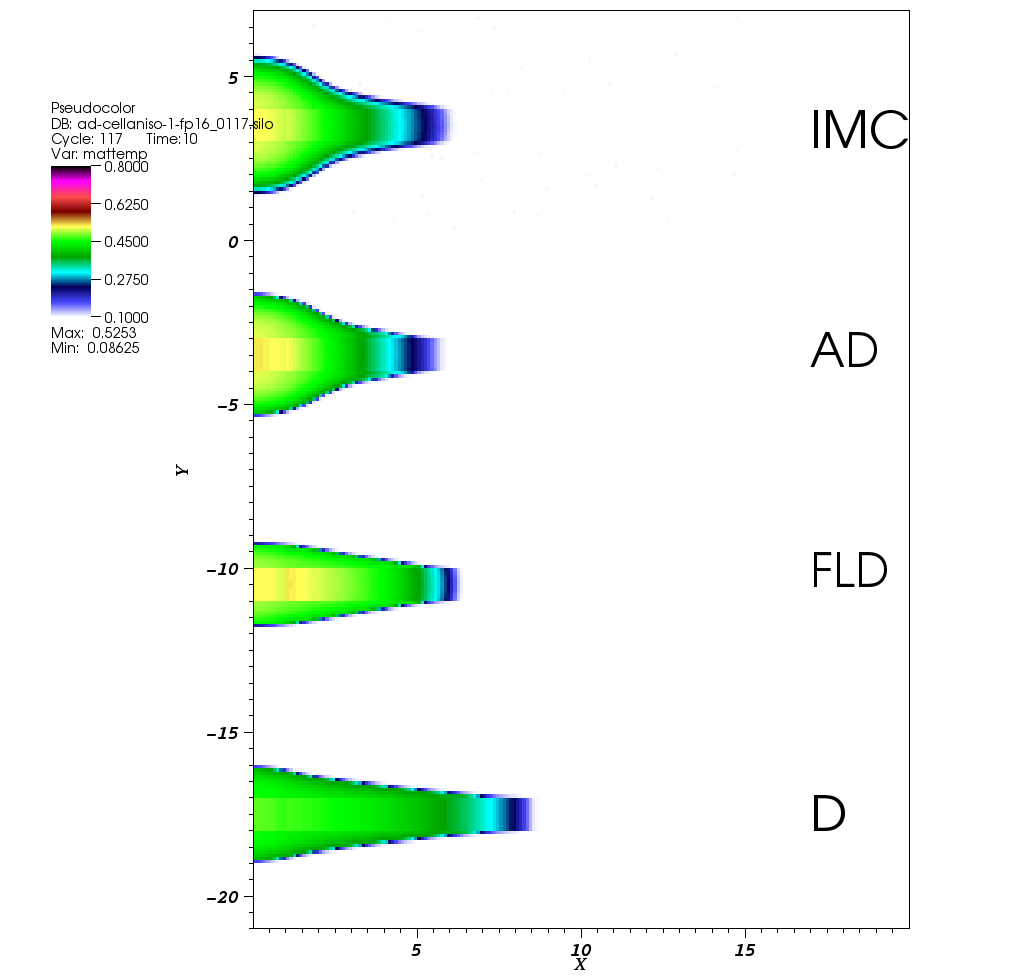
\includegraphics[height=3in]{../figures/crashpipe2b/mattemp/0117}$t=10$}%
\only<10>{\includegraphics[height=3in]{../figures/crashpipe2b/mattemp/0167}$t=15$}%
\only<11>{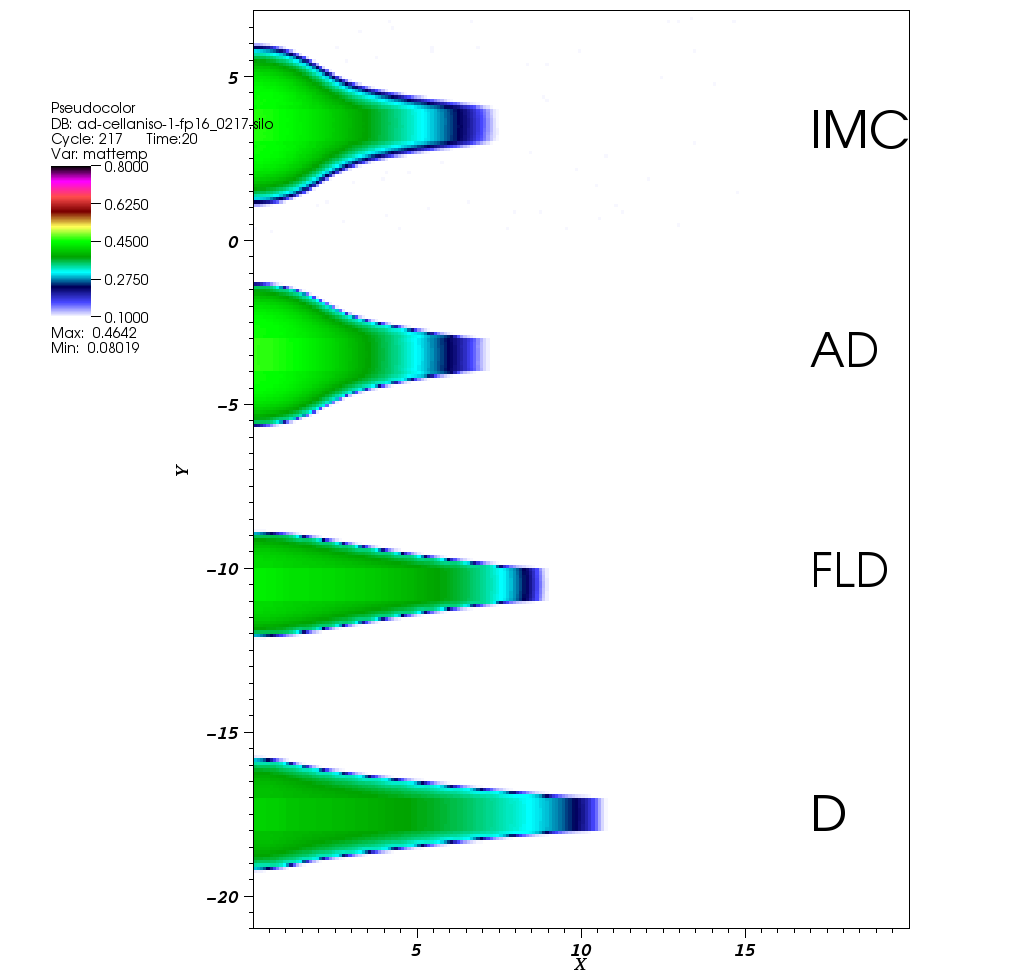
\includegraphics[height=3in]{../figures/crashpipe2b/mattemp/0217}$t=20$}%
\end{frame}
%%%%%%%%%%%%%%%%%%%%%%%%%%%%%%%%%%%%%%%%
\begin{frame}{Time evolution of radiation energy density}

\centering
\hspace{-1in}%
\only<1>{\input{../figures/crashpipe2b/pres-phi-channel-t1/include.tex}}%
\only<2>{\input{../figures/crashpipe2b/pres-phi-channel-t2/include.tex}}%
\only<3>{\input{../figures/crashpipe2b/pres-phi-channel-t5/include.tex}}%
\only<4>{\input{../figures/crashpipe2b/pres-phi-channel-t10/include.tex}}%
\only<5>{\input{../figures/crashpipe2b/pres-phi-channel-t20/include.tex}}%
\hspace{-.35in}
\only<1>{\input{../figures/crashpipe2b/pres-phi-ortho-t1/include.tex}}%
\only<2>{\input{../figures/crashpipe2b/pres-phi-ortho-t2/include.tex}}%
\only<3>{\input{../figures/crashpipe2b/pres-phi-ortho-t5/include.tex}}%
\only<4>{\input{../figures/crashpipe2b/pres-phi-ortho-t10/include.tex}}%
\only<5>{\input{../figures/crashpipe2b/pres-phi-ortho-t20/include.tex}}%
\hspace{-1in}
\par
  
\vspace{-\baselineskip}\small
\only<1>{ $t=1.0$ }%
\only<2>{ $t=2.0$ }%
\only<3>{ $t=5.0$ }%
\only<4>{ $t=10.0$ }%
\only<5>{ $t=20.0$ }%
\end{frame}

%%%%%%%%%%%%%%%%%%%%%%%%%%%%%%%%%%%%%%%%
\begin{frame}{Time evolution of radiation temperature wavefront}
  \centering%
  \input{../figures/crashpipe2b/wavefront-channel/include.tex}%
  \par
\end{frame}
%%%%%%%%%%%%%%%%%%%%%%%%%%%%%%%%%%%%%%%%
\begin{frame}{Diffusion coefficients ($t=10$)}
  \centering%
  \input{../figures/crashpipe2b/pres-dcoeff---channel-t10/include.tex}%
  \par
\end{frame}
%%%%%%%%%%%%%%%%%%%%%%%%%%%%%%%%%%%%%%%%
\begin{frame}{Anisotropic diffusion tensor visualization ($t=10$)}
  \centering%
  \includegraphics[width=.75\textwidth]{../figures/crashpipe2/adcoeff_t10}%
  \par
\end{frame}
%%%%%%%%%%%%%%%%%%%%%%%%%%%%%%%%%%%%%%%%
\begin{frame}{Timing results}
  \begin{table}[htb]
    \centering
    \begin{tabular}{cr}
      Method & Wall time (s) \\ \hline
      IMC & 2730 \\
      FLD & 21 \\
      D   & 20 \\
      AD$_{64}$ & 36 \\
      AD$_{128}$ & 59
    \end{tabular}
    \caption{Approximate run times for pipe test problem with $\Delta_x=0.1$.}
    \label{tab:pipeTiming}
  \end{table}
\end{frame}
%%%%%%%%%%%%%%%%%%%%%%%%%%%%%%%%%%%%%%%%%%%%%%%%%%%%%%%%%%%%%%%%%%%%%%%%%%%%
\section{Conclusions}
%%%%%%%%%%%%%%%%%%%%%%%%%%%%%%%%%%%%%%%%
\begin{frame}
  \frametitle{Conclusions}
  Anisotropic diffusion:
  \begin{itemize}
    \item Accounts for some amount of arbitrary anisotropy in
      angular intensity, unlike standard or flux-limited diffusion, by
      preserving some transport physics
    \item Works best in problems with weaker derivatives, as suggested by
      theory and borne out by numerical experiments
    \item Accurately treats the nonlinear time-dependent flow of radiation
      through a tube like that found in CRASH experiments
  \end{itemize}
\end{frame}
%%%%%%%%%%%%%%%%%%%%%%%%%%%%%%%%%%%%%%%%
\begin{frame}
  \frametitle{Future work}
  \begin{itemize}
    \item Finalize derivation and analysis of transport-matched boundary
      conditions (not presented here).
    \item Implement and test ``Anisotropic P$_1$''
      ($\frac1c\pder{}{t}=O(\epsilon)$ instead of $O(\epsilon^2)$).
    \item Extend the method to anisotropic internal sources.
    \item Keep the $\grad \vd \vec{F}$ term by ignoring assumption of
      $\int_{4\pi} \vec{\Omega} (\cdot) \ud\Omega = O(\epsilon)$.
  \end{itemize}
\end{frame}
%%%%%%%%%%%%%%%%%%%%%%%%%%%%%%%%%%%%%%%%%%%%%%%%%%%%%%%%%%%%%%%%%%%%%%%%%%%%
\appendix
%%%%%%%%%%%%%%%%%%%%%%%%%%%%%%%%%%%%%%%%
\begin{frame}
  \frametitle{Questions?}
  \begin{center}
    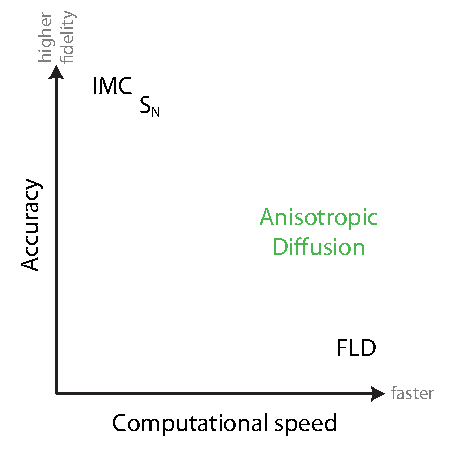
\includegraphics[width=2in]{../figures/fidelity2}
  \end{center}
{\setlength{\baselineskip}{-\baselineskip} \tiny 
This material is based upon work supported under a National Science Foundation
Graduate Research Fellowship and a Department of Energy Nuclear Energy
University Programs Graduate Fellowship. Any opinions, findings, conclusions or
recommendations expressed in this publication are those of the author and do
not necessarily reflect the views of the National Science Foundation or the
Department of Energy Office of Nuclear Energy.\par}
\end{frame}

%%%%%%%%%%%%%%%%%%%%%%%%%%%%%%%%%%%%%%%%
\begin{frame}
  \frametitle{References}
\bibliographystyle{ans}
\bibliography{../SRJall}
\end{frame}
%%%%%%%%%%%%%%%%%%%%%%%%%%%%%%%%%%%%%%%%%%%%%%%%%%%%%%%%%%%%%%%%%%%%%%%%%%%

%	This material is based upon work supported under a National Science
%	Foundation Graduate Research Fellowship. Any opinions, findings, conclusions
%	or recommendations expressed in this publication are those of the author(s)
%	and do not necessarily reflect the views of the National Science
%	Foundation.  
\end{document}
